\chapter{Related Work}\label{cha:2_relatedwork}
Section (\ref{community_in_graph}), describes in brief about community structures in graph and its similarities with real-life. This chapter of the thesis focuses on \textit{state of the art} community detection techniques and explains the algorithms in details. It also focuses on state of the art community detection algorithms and their complexity factors regarding run-time and space. Preceding literature of this chapter unfolds some of the widely used algorithms for community detection and also explores the complexity factors.

\section{Problems of community detection}
Mostly, two paradigms are used to discover the community structure of a network. One of them is based on the analysis of the global features of the network. We can consider network topology as an example. These approaches are characterized by high computational complexity and high-quality results. The other paradigm relies on the local information of the network. For an example of local information would be, information that is acquired by the nodes and their neighbors. The computational cost for these techniques is lower than those exploiting global features but the reliability decreases \cite{ref-28}.

Over the years many techniques have been proposed to detect community structures in large networks. There exist numerous comprehensive surveys of this problem such as \cite{ref-2}, \cite{ref-6}, \cite{ref-9}. The problem of finding communities in a network is intended as a data clustering problem. Two approaches have been widely investigated over the time for community detection in networks,
\begin{itemize}
	\item \textit{Spectral Clustering}
	\item \textit{Network Modularity Optimization} 
\end{itemize}
\textit{Spectral clustering} uses the optimization of the process of cutting the graph that represents the network and \textit{Modularity optimization} focuses on maximizing the modularity (quality function) of the network. For the first process, the problem of minimizing the number of cuts in a given graph has been proven to be NP-hard \cite{ref-29}. The main issue with spectral clustering based method is that one has to know in advance the number and the size of communities in a given graph representing a network. In large networks, this method is not feasible.

As for modularity optimization relies on a concept called network modularity. Network modularity is explained in details in this chapter earlier. Equation (\ref{sumoverclusters}) reveals a possible maximization strategy: in order to increase the value of first term, the highest possible number of edges should fall in each given community, whereas the minimization of the second term is obtained by dividing the network into several communities with small total degrees. The problem of maximizing the network modularity had been proven to be NP-Complete \cite{ref-30}. Several heuristic strategies have been proposed so far. (\ref{girvan-newman}) and (\ref{sub:fastalgorithm}) proposed by \textit{Girvan-Newman} are probably the most popular strategy to determine communities in a given graph representing a network. When considering a strategy to compute and detect communities, it's important to consider the resource needed and time for completing the computation. The computational cost for modularity maximization is high. It yields $\mathcal{O}(n^{3})$ where $n$ is the number of nodes. In this process, the largest part of the cost is given to calculate \textit{betweenness centrality}. Betweenness centrality is explained in brief in this chapter earlier in section (\ref{betweennesscentrality}).

Several variations of this strategy have been proposed and all of them were focused on faster calculation and detection on communities. The fast clustering algorithm by \textit{Clauset, Newman and Moore} \cite{ref-31}, that runs in $\mathcal{O}(n \log n)$ on sparse graphs; the external optimization method proposed by Duch and Arenas \cite{ref-32}, based on fast agglomerative approach, with $\mathcal{O}(n^2 \log n)$ time complexity; the Newman-Leicht \cite{ref-33} mixture model based on statistical inferences. Maximization techniques by Newman \cite{ref-34} based on eigenvectors and matrices.

\section{Literature Review}\label{sec:literature_review}
Over the past years, network research across the physical and social sciences grew very fast\cite{ref-25}. As a result, there are several techniques to determine community structure in a network. Finding communities within an arbitrary network can be a computationally difficult task. The number of communities, if any, within a network, is generally unknown and communities are often unequal in size or density. Despite these difficulties, however, several methods for community finding have been developed and employed with varying levels of success \cite{ref-2}. Following is a list of few well known community detection algorithms for large-scale networks and this chapter of the thesis is focused on technical aspects of these algorithms for community detection in large-scale networks.

\begin{enumerate}
	\item InfoMap
	\item Louvain Method
	\item Girvan-Newman algorithm
    \item Modularity maximization (Quality Function)
    \item Hierarchical clustering
	\item Graph partitioning
	\item Minimum cut method
	\item Statistical inference
	\item Clique-based methods
\end{enumerate}

These algorithms are chosen because of the nature of their performance against large-scale networks. According to the authors of these algorithms each one of them is fast and optimized for community detection. Authors of each algorithm has chosen different approach to detect communities in large-scale networks. Next section will attempt an ordered exposition of the fundamental concepts of some of these algorithms to explore the ideas and technical background behind these community detection algorithm in respect to large-scale transaction-based network. Although all the algorithm mentioned above are deemed fast enough at the time of their publications, some of them might not be suited for detecting community structures in large-scale transaction-based network. In chapter (\ref{cha:4_implementation_and_evaluation}), these algorithms will be evaluated with a prototypical framework for detecting communities in distributed ledger network.

\subsection{Infomap}\label{subsec:infomap}
Communities refer to groups of nodes that are densely connected internally. Community detection in networks is challenging, and many algorithms have been proposed in the last few years to tackle this difficult problem. The current implementation of Infomap is both fast and accurate \cite{ref-42}. It can classify millions of nodes in minutes and performs very well on synthetic data with planted communities. Furthermore, the map equation framework is also naturally flexible and can be straightforwardly generalized to analyze different kinds of network data \cite{ref-42}. Infomap uses, map equation \cite{ref-43} first introduced by Martin et. al in 2009. The map equation is a Flow-based method. Methods based on flows operate on the dynamics on the network rather than on its topological structure per se. The rationale is that the prime function of networks is to capture the flow between the components of the real systems they represent. Accordingly, communities consist of nodes among which flow persists for a long time once entered \cite{ref-42}. Map equation uses \textit{Huffman coding} \cite{ref-44} to send the location of the random walker \cite{ref-57} in the flow. Moreover, it is optimal for describing a list of locations of the random walker at arbitrary (and sufficiently distant) times. However, it can be used to list the locations visited by a random walker in a sequence of successive steps, after all this is the flow of the network \cite{ref-43}. 

\subsection{Louvain Method}\label{subsec:louvain_method}
\textit{Louvain Method} (henceforth, LM) was first introduced by Bodel et al. in 2008 in \cite{ref-27}. The authors in this publication proposed a simple method to extract the community structure of large networks. The proposed method is a heuristic method that is based on modularity optimization (\ref{sumoverclusters}). LM has outperformed all other known community detection methods in terms of computation time \cite{ref-28}. The subject of computation time of different community detection algorithms will be discussed in a comparative manner later in this chapter. Moreover, depending on modularity function, community detected by LM is very good. The authors introduced an algorithm that is capable of detecting high modularity partitions of large networks in a short time and it also unfolds a complete hierarchical community structure for the network. This unfolding process of unfolding structure gives access to different levels of resolutions of community detection. Authors have tested the algorithm with 118 million nodes network which took only 152 minutes\footnote{All methods described in \cite{ref-27} have been compiled and tested on the same machine: a biopteron
2.2k with 24GB of memory} \cite{ref-27}. In 2011, Meo et al. in \cite{ref-28} proposed a generalized LM for community detection in large network with a brief discussion of core LM \cite{ref-27} and with the help of the state of the art LM and $\mathcal{K}$-path edge centrality, message propagation and fast $\mathcal{K}$-path community detection. In this recent paper the authors have shown that their algorithm outperforms all the other community detection algorithms and also slightly improves the core LM \cite{ref-28}.

\subsection{Girvan-Newman Algorithm}\label{girvan-newman}
The most popular algorithm for community structure detection was proposed by Girvan and Newman \cite{ref-1}. This algorithm marked the new era in community detection. Here edges are selected according to the values of measures of \textit{edge centrality}, estimating the importance of the edge according to some property or process running on the graph. Girvan and Newman focused on the concept of \textit{betweenness} (\ref{betweennesscentrality}), which is a variable expressing the frequency of the participation of edges to a process. They considered three alternative definitions: \textit{geodesic edge betweenness}, \textit{random-walk edge betweenness} and \textit{current-flow edge betweenness} \cite{ref-6}. Edge betweenness is highest for the edge connecting communities. In the Figure (\ref{edgebetweenness}) the edge in the middle has a much higher betweenness than all the other edges. The algorithm stated in \cite{ref-1} is as follows:

\begin{enumerate}
	\item Calculate the betweenness for all edges in the network.
	\item Remove the edge with the highest betweenness.
	\item Recalculate betweenness for all edges affected by the removal.
	\item Repeat from step 2 until no edges remain.
\end{enumerate}

\subsection{Modularity Maximization (Quality Function)}
Algorithms for community detection are supposed to identify \textit{good} partitions. The question remains, what is a good clustering? In order to distinguish between a ``good" and ``bad" clustering, it would be useful to require that partitions satisfy a set of basic properties. In \cite{ref-14}, J. Kleinberg proved an \textit{impossibility theorem} in the field of data clustering.

Given a set $S$ of points, a \textit{distance function} $d$ is defined, which is positive definite and symmetric (the triangular inequality is not explicitly required). One wishes to find a \textit{clustering} $f$ based on the distances between the points. Kleinberg showed that \textbf{no clustering} can satisfy the following three properties at the same time.

\begin{enumerate}
	\item \textit{Scale-invariance}: given a constant $\alpha$, multiplying \textit{any} distance function $d$ by $\alpha$ yields the same clustering.
	\item \textit{Richness}: any possible partition of the given point set can be recovered if one chooses a suitable distance function $d$.
	\item \textit{Consistency}: given a partition, any modification of the distance function that does not decrease the distance between points of different clusters and that does not increase the distance between points of the same cluster, yields the same clustering.
\end{enumerate}

The theorem cannot be extended to graph clustering because the distance function cannot be in general defined for a graph which is not complete. For weighted complete graph, like  correlation matrices \cite{ref-15}, it is often possible to define distance function. On a generic graph, except for the first property, which does not make any sense without distance function,\footnote{The traditional shortest path distance between vertices is not suitable here, as it is integer by definition} the other two are quite well defined.

The property of richness implies, given a partition, edges can be set between the vertices in such a way that the partition is a natural outcome of the resulting graph (e.g., it could be achieved by setting edges only between vertices of the same cluster). Consistency here implies that deleting inter-cluster edges and adding intra-cluster edges yields the same partition.

% ================================================================================================= %

\section{Background}
In previous section (\ref{sec:literature_review}) of this thesis, some of the community detection algorithms have been introduced and discussed in brief. This section will focus on the technical backgrounds, mathematics and equations that explains the algorithms described in section (\ref{sec:literature_review}).

\subsection{Infomap Algorithms}\label{infomap_algorithms}
Infomap optimizes the map equation, which exploits the information-theoretic duality between the problem of compressing data, and the problem of detecting and extracting significant patterns or structures within those data. Infomap captures flow patterns modeled with both first-order dynamics (as on a conventional network: where flow moves to on the network only depends on where it currently is) and second-order dynamics (where flow moves to on the network both depends on where it currently is and where it just came from). Infomap
captures second-order dynamics by performing first-order dynamics on memory nodes \cite{ref-46}. The calculation process of Infomap algorithm is divided into two steps. First, The communities and nodes are coded respectively by the algorithm, the coding length is minimized, where $n$ is the number of nodes in the network, the computable complexity is $\mathcal{O}(n^3)$. Secondly, the modularity of the community detection is optimized by simulated annealing algorithm. This method can reduce the previous time complexity into $\mathcal{O}(n^2)$ \cite{ref-48}.

\subsubsection*{Map Equation}\label{subsec:map_equation}
Map equation provides the theoretical limit of how concisely the network path is specified using a given partition structure. To find an optimal partition of the network, it is sufficient to calculate this theoretical limit for different partitions of the network and pick the one that gives the shortest description length.

For a module $M$ of $n$ nodes $\alpha = 1,2,3,...,n$ into $m$
modules $i = 1,2,3,.....,m$, defined as the lower bound on code length to be $L(M)$. To calculate $L$ for an arbitrary partition, Shanon's source coding theorem \cite{ref-45} is invoked. Which implies that, use of $n$ codewords to describe the $n$ states of a random variable $X$ that occur with frequency $\mathcal{P}_i$, the average length of a codeword can be no less than the entropy of the random variable $X$ itself:
$H(X) = \sum_{1}^{n}\mathcal{P}_i log(\mathcal{P}_i)$
To calculate the average length of the code describing a step of the random walk, weight of average length is needed from the index codebook ({refer to \cite{ref-44} and \cite{ref-43}}) and module codebooks by their rates of use. The map equation is:

\begin{equation}\label{eq:infomap_map_equation}
L(\mathcal{M}) = q_\curvearrowright H(\mathcal{Q}) + \sum_{i=1}^m \mathcal{P}_\circlearrowright^i H(\mathcal{P}^i)
\end{equation}
Here $H(\mathcal{Q})$ is the frequency-weighted average length of codewords in the index codebook and $H(\mathcal{P}^i)$ is the frequency-weighted average length of codewords in the module codebook $i$. Further, the entropy terms are weighted by the rate at which the codebooks are used. With $q_{i\curvearrowright}$ for the probability to exit module $i$, the index codebook is used at a rate $q_{\curvearrowright} = \sum_{i=1}^{m} q_{i\curvearrowright}$, the probability that the random walker switches modules on any given step. With $p_\alpha$ for the probability to visit node $\alpha$, module codebook $i$ is used at a rate $p_{\curvearrowright}^i = \sum_{\alpha \in i} p\alpha + q_{i\curvearrowright}$, the fraction of time the random walk spends in module $i$ plus the probability that it exits the module and the exit message is used. Now it is straightforward to express the entropies in $q_{i\curvearrowright}$ and $p\alpha$. For the index codebook, the entropy is

\begin{equation}\label{eq:infomap_index_entropy}
H(\mathcal{Q}) = - \sum_{i=1}^{m} \dfrac{q_{i\curvearrowright}}{\sum_{j=1}^{m}q_{j\curvearrowright}} log \left(\dfrac{q_{i\curvearrowright}}{\sum_{j=1}^{m} q_{j\curvearrowright}}\right)
\end{equation}
and for module codebook $i$ the entropy is

\begin{equation}\label{eq:infomap_codebook_entropy}
H(\mathcal{P}^i) = - \dfrac{q_{i\curvearrowright}}{q_{i\curvearrowright} + \sum_{\beta \in i} p_\beta} log \left(\dfrac{q_{i\curvearrowright}}{q_{i\curvearrowright} + \sum_{\beta \in i} p_\beta}\right) - \sum_{\alpha \in i} \dfrac{p_\alpha}{q_{i\curvearrowright} + \sum_{\beta \in i}} log \left(\dfrac{p_\alpha}{q_{i\curvearrowright} + \sum_{\beta \in i}}\right)
\end{equation}
By combining Equations (\ref{eq:infomap_index_entropy}) and (\ref{eq:infomap_codebook_entropy}) and simplifying, the map equation (\ref{eq:infomap_map_equation}) takes the following form:
\begin{align}
L(\mathcal{M}) &= \left(\sum_{i=1}^{m} q_{i\curvearrowright}\right) log \left(\sum_{i=1}^{m} q_{i\curvearrowright}\right) - 2 \sum_{i=1}^{m} q_{i\curvearrowright} log (q_{i\curvearrowright}) \nonumber \\
&- \sum_{\alpha=1}^{n} p_\alpha log (p_\alpha) + \sum_{i=1}^{m} \left(q_{i\curvearrowright} + \sum_{\alpha \in i} p_\alpha\right) log \left(q_{i\curvearrowright} + \sum_{\alpha \in i} p_\alpha\right)
\end{align}
In this expended form of the map equation, the term $\sum_{\alpha=1}^{n} p_\alpha log (p_\alpha)$ is independent of partitioning, and elsewhere in the expression $p_\alpha$ appears only when summed over all nodes in a module.

The node visit of node $\alpha$ simply corresponds to the relative weight $W_\alpha$ of the links connected to the node considering the network is undirected. The relative weight is the total weight of the links connected to the node divided by twice the total weight of all links in the network, which corresponds to the total weight of all link-ends. With $W_\alpha$ for the relative weight of node $\alpha$, $w_i = \sum_{\alpha \in i}w_\alpha$ for the relative weight of module $i$, $w_{i\curvearrowright}$ for the relative weight of links exiting module $i$, and $w_{\curvearrowright} = \sum_{i=1}^{m} w_{i\curvearrowright}$ for the total relative weight of links between modules, the map equation is as follows:

\begin{align}
L(\mathcal{M}) &= w_{\curvearrowright} log(w_\curvearrowright) -2\sum_{i=1}^{m} w_{i\curvearrowright} log(w_{i\curvearrowright}) \nonumber \\ &- \sum_{\alpha=1}^{n} w_\alpha log(w_\alpha) + \sum_{i=1}^{m} (w_{i\curvearrowright} + w_i) log(w_{i\curvearrowright} + w_i)
\end{align}

\subsubsection*{Two-level Algorithm}\label{subsubsec:two_level_algorithm}
The core of the algorithm follows closely the Louvain method (\ref{subsec:louvain_method}): neighboring nodes are joined into modules, which subsequently are joined into super-modules and so on. First, each node is assigned to its own module. Then, in random sequential order, each node is moved to the neighboring module that results in the largest decrease of the map equation. If no move results in a decrease of the map equation, the node stays in its original module. This procedure is repeated, each time in a new random sequential order until no move generates a decrease of the map equation. Now the network is rebuilt, with the modules of the last level forming the nodes at this level, and, exactly as at the previous level, the nodes are joined into modules. This hierarchical rebuilding of the network is repeated until the map equation cannot be reduced further.

With this algorithm, a fairly good clustering of the network can be found in a very short time. This algorithm is called the core algorithm. The nodes assigned to the same module are forced to move jointly when the network is rebuilt. As a result, what was an optimal move early in the algorithm might have the opposite effect later in the algorithm. Because two or more modules that merge together and form one single module when the network is rebuilt can never be separated again in this algorithm, the accuracy can be improved by breaking the modules of the final state of the core algorithm in either of the two following ways:

\textit{Sub-module movements}: First, each cluster is treated as a network on its own and the main algorithm is applied to this network. This procedure generates one or more sub-modules for every module. Then all sub-modules are moved back to their respective modules of the previous step. At this stage, with the same partition as in the previous step but with each sub-module being freely movable between the modules, the main algorithm is re-applied on the sub-modules.

\textit{Single-node movements}: First, each node is re-assigned to be the sole member of its own module, in order to allow for single-node movements. Then all nodes are moved back to their respective modules of the previous step. At this stage, with the same partition as in the previous step but with each single node being freely movable between the modules, the main algorithm is re-applied on the single nodes.
In practice, the two extensions are repeated to the core algorithm in sequence and as long as the clustering is improved. Moreover, the sub-module movements are applied recursively. That is, to find the sub-modules to be moved, the algorithm first splits the sub-modules into sub-sub-modules, sub-sub-sub-modules, and so on until no further splits are possible. Finally, because the algorithm is stochastic and fast, we can restart the algorithm from scratch every time the clustering cannot be improved further and the algorithm stops. The implementation is straightforward and, by repeating the search more than once, 100 times or more if possible, the final partition is less likely to correspond to a local minimum. For each iteration, the clustering is recorded if the description length is shorter than the previously shortest description length \cite{ref-47}.

\subsubsection*{Multilevel Algorithm}\label{subsubsec:multilevel_algorithm}
Infomap uses generalized search algorithm for the two-level map equation to recursively search for multilevel solutions. The recursive search operates on a module at any level; this can be all the nodes in the entire network or a few nodes at the finest level. For a given module, the algorithm first generates sub-modules if this gives a shorter description length. If not, the recursive search does not go further down this branch. But if adding sub-modules gives a shorter description length, the algorithm tests if movements within the module can be further compressed by additional index codebooks. Further compression can be achieved both by adding one or more coarser codebooks to compress movements between sub-modules or by adding one or more finer index codebooks to compress movements within sub-modules. To test for all combinations, the algorithm calls itself recursively, both operating on the network formed by the sub-modules and on the networks formed by the nodes within every sub-module. In this way, the algorithm successively increases and decreases the depth of different branches of the multilevel code structure in its search for the optimal hierarchical partitioning. For every split of a module into sub-modules, the two-level search algorithm (\ref{subsubsec:two_level_algorithm}) described above is being used \cite{ref-47}.

% ============================================================================================== %

\subsection{Louvain Method Algorithm Structure}\label{subsec:generalized_louvain}
\textit{Louvain Method} \cite{ref-27} is a strategy based on local information and well suited for analyzing large weighted networks. It is based on two simple steps:
\begin{itemize}
	\item Each node is assigned to a community chosen in order to maximize the network modularity $Q$
	\item Creating a new network consisting of nodes that are those communities previously found
\end{itemize}
The algorithm's efficiency results from the fact that the gain in modularity $\Delta Q$ obtained by moving an isolated node $i$ into a community $C$ can easily be computed by \cite{ref-27}
\begin{equation}
\Delta Q = \left[\dfrac{\sum_{in} + k_{i,in}}{2m} - \left( \dfrac{\sum_{tot} + k_i}{2m}\right)^2\right] - \left[\dfrac{\sum_{in}}{2m} - \left(\dfrac{\sum_{tot}}{2m}\right)^2 - \left(\dfrac{k_i}{2m}\right)^2\right]
\end{equation}
where $\sum_{in}$ is the sum of the weights of the links inside $C$, $\sum_{tot}$ is the sum of the weights of the links incident to nodes in $C$, $k_i$ is the sum of the weights of the links incident to node $i$, $k_{i,in}$ is the sum of the weights of the links from $i$ to the nodes in $C$ and $m$ is the sum of the weights of all the links in the network. The edge weighting is based on the $\mathcal{K}$-path edge centrality, an approach whose calculation requires a near linear computational cost \cite{ref-35}.

\subsubsection*{$\mathcal{K}$-Path Edge Centrality}\label{sec:k-path-edge-centrality}
For each edge $e$ of a graph $G = \langle V, E\rangle$, the $\mathcal{K}$-path edge centrality $L^k(e)$ of $e$ is defined as the sum, over all possible source nodes $s$, of the frequency with which a message originated from $s$ traverses $e$, assuring that the message traversals are only along random simple paths of at most $k$ edges \cite{ref-35}.
The $\mathcal{K}$-path edge centrality is formalized, for an arbitrary edge $e$, as follows
\begin{equation}\label{k-path-edge-centrality}
L^k(e) = \sum_{s \in V} \dfrac{\sigma_s^k(e)}{\sigma_s^k}
\end{equation}
where $s$ are all the possible source nodes, $\sigma_s^k(e)$ is the number of $\mathcal{K}$-paths originating from $s$ and traversing the edge $e$ and, finally, $\sigma_s^k$ is the number of $\mathcal{K}$-paths originating from $s$.

In practical cases, the application of equation (\ref{k-path-edge-centrality}) cannot be feasible because it requires to count all the $\mathcal{K}$-paths originating from all the source nodes $s$ and such number can be exponential in the number of nodes of $G$. To this purpose, authors in \cite{ref-35} designed algorithms capable of efficiently approximating the value of $\mathcal{K}$-path edge centrality.

The algorithm called \textit{Edge Random Walk $\mathcal{K}$-Path Centrality} (or in short, ERW-KPath)for computing $\mathcal{K}$-path edge centrality consists of two main steps:\\ \textit{(i)} node and edge weights assignment\\ 
\textit{(ii)} simulation of message propagation through random simple paths.

\subsubsection*{\textit{Node and edge weights assignment}}
In the first step of the algorithm, weight is assigned to both nodes and edges of the graph $G = \langle V, E \rangle$ representing the network. Weights on nodes are used to select source nodes from which message propagation simulation starts. Weights on the edges represent initial values of edge centrality and to comply with the second \textit{(ii)} step of the algorithm they will update during the execution of the algorithm. To compute weights on the nodes, authors in  \cite{ref-35} has introduced the \textit{normalized degree} $\delta(v_n)$ of a node $v_n \in V$ as follows:\\\\
\textbf{\textit{Normalized Degree:}}\\
Given an undirected graph $G = \langle V, E \rangle$ and a node $v_n \in V$, its normalized degree $\delta(v_n)$ is
\begin{equation}\label{k-path-normalized-degree}
\delta (v_n) = \dfrac{\mid I(v_n) \mid}{\mid V \mid}
\end{equation}
where $I(v_n)$ represents the set of edges incidents on $v_n$. The normalized degree $\delta(v_n)$ correlates the degree of $v_n$ and the number of total nodes on the network. It also represents that how much a node contributes to the overall connectivity of the graph. Its value belongs to the interval of $\left[0,1\right]$ and the higher $\delta (v_n)$, the better $v_n$ is connected to the graph.\\\\
\textbf{\textit{Initial edge weight:}}\\
Given an undirected graph $G = \langle V, E \rangle$ and an edge $e_m \in E$, its initial edge weight $\omega_0 (e_m)$ is
\begin{equation}\label{initial-edge-weight}
\omega_0(e_m) = \dfrac{1}{\mid E \mid}
\end{equation}
The meaning of equation (\ref{initial-edge-weight}) is as follows: an initial "BUDGET" consisting of $\mid E \mid$ points; these points are equally divided among all the possible edges; the amount of points received by an edge represents its initial rank. Figure (\ref{fig:initial-edge-weight-graph}) shows an example of graph $G$ along with the distribution of weights on nodes and edges.
\begin{figure}[!ht]
	\centering
	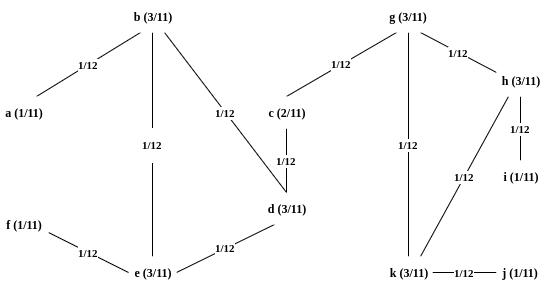
\includegraphics[width=0.8\textwidth]{k-path-initial-weights}
	\caption{Example of assignment of normalized degrees and initial edge weights \cite{ref-35}.}
	\label{fig:initial-edge-weight-graph}
\end{figure}

\subsubsection*{\textit{Simulation of message propagation through random simple $\mathcal{K}$-paths}}
In the second step authors of \cite{ref-35} has introduced $\rho$ simple random walks of length at most $\mathcal{K}$ on the network. The ERW-$\mathcal{K}$-path algorithm performs the following operations at each iteration.
\begin{enumerate}
	\item A node $v_n \in V$ of the graph $G$ is selected according to one of the following two possible strategies:
	\begin{enumerate}[label=\alph*.]
		\item uniformly at random, with a probability:
		\begin{equation}
		P(v_n) = \dfrac{1}{\mid V \mid}
		\end{equation}
		\item with a probability proportional to its normalized degree $\delta(v_n)$, given by:
		\begin{equation}\label{probability-of-normalized-degree}
		P(v_n) = \dfrac{\delta(v_n)}{\sum_{v_k \in V} \delta(v_k)}
		\end{equation}
	\end{enumerate}
	\item All the edges in $G$ are marked as not traversed
	\item The procedure \textit{MessagePropagation} is invoked
\end{enumerate}
\textbf{\textit{MessagePropagation:}}\\
This very procedure carries out a loop as long as \textit{both} the following conditions hold true:
\begin{itemize}
	\item The length of the path currently generated is no greater than $k$. This is managed through a length counter $N$
	\item Assuming that the walk has reached the node $v_n$, there must exist at least an incident edge on $v_n$ which has not been already traversed. To do so, a flag $T(e_m)$ is attached to each edge $e_m \in E$, such that
	\begin{equation}
	T(e_m) = \begin{cases}
	1 & \text{if $e_m$ has already been traversed}\\
	0 & \text{otherwise}
	\end{cases} 
	\end{equation}
	the following condition must hold true:
	\begin{equation}
	\mid I(v_n) \mid \quad > \sum\limits_{e_k \in I(v_n)} T(e_k)
	\end{equation}
	being $I(v_n)$ the set of edges incident onto $v_n$.
\end{itemize}
If the conditions above are satisfied, the \textit{MessagePropagation} procedure selects an edge $e_m$ by applying two strategies:
\begin{enumerate}[label=\alph*.]
	\item uniformly at random, with probability
	\begin{equation}
	P(e_m) = \dfrac{1}{\mid I(v_n) \mid - \sum\limits_{e_k \in I(v_n)} T(e_k)}
	\end{equation}
	among all the edges $e_m \in \left\{ I(v_n) | T(e_m) = 0\right\}$ incident on $v_n$ (i.e., excluding already traversed edges)
	\item with a probability proportional to the edge weight $\omega_l (e_m)$, given by
	\begin{equation}\label{probability-edge-weight}
	P(e_m) = \dfrac{\omega_l (e_m)}{\sum\limits_{e_m \in \hat{I}(v_n)} \omega_l (e_m)}
	\end{equation}
	being $\hat{I}(v_n) = \{e_k \in I(v_n) | T(e_k) = 0\}$ and $\omega_l (e_m) = \omega_{l-1} (e_m) + \beta \cdot T(e_m)$ if $1 \le l \le k\rho$
\end{enumerate}
Let $e_m$ be the selected edge and let $v_{n+1}$ be the node reached from $v_n$ by means of $e_m$. The \textit{MessagePropagation} procedure awards a bonus $\beta$ to $e_m$, sets $T(e_m) = 1$ and increases the counter $N$ by 1. The message propagation activity continues from $v_{n+1}$.

\begin{algorithm}[ht!]
	\caption{WERW-$\mathcal{K}path$(Graph $G = \langle V, E\rangle$, int $k$, int $\rho$, float $\beta$)}
	\label{algo:werw-kapth-algorithm}
	\SetAlgoLined
	\DontPrintSemicolon
	Assign each node $v_n \in V$ its normalized degree\;
	Assign each edge $e_m \in E$ the uniform probability function as weight\;
	\For{$i=1$ to $\rho$}{
		$N \gets 0$ a counter to check the length of the $k$-path\;
		$v_n \gets $ a node chosen uniformly at random in $V$\;
		MessagePropagation($v_n$, $N$, $k$, $\beta$)
	}
\end{algorithm}
\begin{algorithm}[ht!]
	\caption{MessagePropagation(Node $v_n$, int $N$, int $k$, float $\beta$)}
	\label{algo:message-propagation-algorithm}
	\SetAlgoLined
	\DontPrintSemicolon
	\While{$N < k$ and $\left[ \mid I(v) \mid > \sum_{e \in I(v)} T(e)\right]$}{
		$e_m \gets e_m \in \left\{I(v) | T(e_m) = 0\right\}$, chosen uniformly at random\;
		Let $v_{n+1}$ be the node reached by $v_n$ through $e_m$\;
		$\omega (e_m) \gets \omega (e_m) + \beta$\;
		$T(e_m) \gets 1$\;
		$v_n \gets v_{n+1}$\;
		$N \gets N + 1$\; 
	}
\end{algorithm}
Algorithm (\ref{algo:werw-kapth-algorithm}) and algorithm (\ref{algo:message-propagation-algorithm}) described in this section adopts uniform probability distribution functions in order to choose nodes and edges purely at random and as discussed before it is called ERW-$\mathcal{K}$path. Although, a weighted version of the same algorithm, called WERW-$\mathcal{K}$path, both algorithms would differ only in line 5,  adopting weighted functions specified in Equations (\ref{probability-of-normalized-degree}) and (\ref{probability-edge-weight}).

The time complexity if the ERW-$\mathcal{K}$Path algorithm is $\mathcal{O}(\kappa \rho)$. If, $\rho = \mid E \mid - 1$, then algorithm achieves a good trade off between accuracy and computational costs. In fact, in such a case, the worst case time complexity of ERW-$\mathcal{K}$Path algorithm is $\mathcal{O}(\kappa \mid E \mid)$.

\subsubsection*{Fast $\mathcal{K}$-Path Community Detection}
In \cite{ref-28}, Meo et al. introduced a generalized LM \cite{ref-27} that outperforms other community detection techniques and also slightly improves results of the original LM. Authors of \cite{ref-28} named their proposed algorithm as \textit{Fast $\mathcal{K}$-Path Community Detection} (or shortly, FKCD), hence-forth FKCD. This particular algorithm inhabits the main features of the original LM and relies on three steps:\\\\
\textit{(i)} Ranking edges by using the WERW-$\mathcal{K}$path algorithm\\
\textit{(ii)} Calculating the proximity (the inverse of the distance) between each pair of connected nodes\\
\textit{(iii)} Partitioning the network into communities so to optimize the network modularity \cite{ref-1}

\subsubsection*{Ranking Edges by Using WERW-$\mathcal{K}$path}
FKCD algorithm requires a ranking criterion to compute the aptitude of all the edges to propagate information through the network. To do so, FKCD invokes the WERW-$\mathcal{K}$path algorithm (\ref{sec:k-path-edge-centrality}). Once all the edges have been labeled with their $\mathcal{K}$-path edge centrality, a ranking in decreasing order of centrality could be obtained. The computational cost of this step is $\mathcal{O} (\kappa \mid E \mid)$, with $k$ length of the $\mathcal{K}$-paths and $\mid E \mid$ cardinality of $E$.

\subsubsection*{Calculation of Proximity Between Each Pair of Connected Nodes}
In the second step, FKCD calculates the proximity of each connected pair of nodes using a $L_2$ distance, commonly known as \textit{Euclidean distance} which has been discussed briefly in this thesis in section (\ref{vertexsimilarity}). $L_2$ distance for FKCD is calculated as:
\begin{equation}\label{eq:node-proximity}
r_{ij} = \sqrt{\sum_{\kappa = 1}^{n} \dfrac{(L^\kappa (e_{i \kappa}) - L^\kappa (e_{\kappa j}))^2}{d(\kappa)}}
\end{equation}
where $L^\kappa(e_{i \kappa})$ (resp., $L^\kappa(e_{\kappa j})$) is the $kappa$-path edge-centrality of the edge $e_{i \kappa}$ (resp., $e_{\kappa j}$) and $d(\kappa)$ is the degree of the node.

Even though $L_2$ measure would return a distance, in this case, the higher $L^\kappa (e_{i \kappa})$ (resp., $L^\kappa (e_{\kappa j})$), the more the nodes are near, instead of distance. This step of FKCD algorithm is theoretically computationally expensive because it should require $\mathcal{O} (\mid V \mid^2)$ iterations. But in practice, by adopting optimization techniques, its near-linear computation cost is $\mathcal{O} (\bar{d}(v) \mid V \mid)$, where $\bar{d}(v)$ is the mean degree of all the nodes of the network (it's usually small in very large networks) \cite{ref-28}.

\subsubsection*{Network Partitioning}\label{subsec:network-partitioning}
The principal idea of network partitioning is inspired by the LM \cite{ref-27} for detecting the community structure of weighted networks in a near linear time. Network partitioning is an iterative process. At each iteration FKCD repeats two simple steps:\\\\
\textit{(i)} Each node is assigned to a community chosen in order to maximize the network modularity $Q$. This process has been discussed explicitly in section (\ref{sebsec:modularity-optimization}).\\
\textit{(ii)} The second step produces a \textit{meta-network} whose nodes are those communities previously found.
partitioning ends when no further improvements of $Q$ can be obtained.

For this third step, cost of computation is $\mathcal{O} (\gamma \mid V \mid)$, where $\mid V \mid$ is the cardinality of $V$ and $\gamma$ is the number of iterations required by the algorithm to converge (usually, $\gamma < 5$) \cite{ref-28}.

\begin{algorithm}
	\caption{FKCD(Graph $G = (V, E)$, int $\kappa$)}
	\label{algo:fkcd-algorithm}
	\SetAlgoLined
	\DontPrintSemicolon
	WERW-Kpath(G, $\kappa$)\tcp*{Using algorithm (\ref{algo:werw-kapth-algorithm})}
	CalculateDistance(G)\tcp*{Calculates distance with Eq. (\ref{eq:node-proximity})}
	\While{$Q$ increases at least of $\in$ (arbitrarily small)}{
		$P = $ Partition(G)\tcp*{Partitioning is done with (\ref{subsec:network-partitioning})}
		$Q \gets $ NetworkModularity(P)\tcp*{Measures modularity with Eq. (\ref{sumoverclusters})}
	}
\end{algorithm}
The computational cost for the whole strategy described in this algorithm is near linear. In fact, $\mathcal{O} (\kappa \mid E \mid + \;\bar{d} (e) \mid V \mid + \;\gamma \mid V \mid) = \mathcal{O} (\tau \mid E \mid)$, by adopting efficient graph memorization in order to minimize the execution time for the computation of Equations (\ref{sumoverclusters}) and (\ref{eq:node-proximity}).

\vfill
\pagebreak

% ================================================================================================= %

\subsection{Girvan-Newman Algorithm Architecture}
\textit{Edge betweenness} is the number of shortest paths between all vertex pairs that run along the edge. It is an extension to edges of the popular concept of site betweenness, introduced by Freeman \cite{ref-11} and expresses the importance of edges in processes like information spreading, where information usually spreads through the shortest paths. It is intuitive that inter-community edges have a large value of the edge betweenness, because many \textit{shortest paths} connecting vertices of different communities will pass through them (\ref{edgebetweenness}). If there are two or more geodesic paths with the same endpoints that run through an edge, the contribution of each of them to the betweenness of the edge must be divided by the multiplicity of the paths. The betweenness of all edges of the graph can be calculated in a time that scales as $\mathcal{O}(mn)$, or $\mathcal{O}(n^2)$ on a sparse graph, with techniques based on breadth-first-search \cite{ref-12}.

In the context of information spreading, it is very common and realistic that signals flow across random rather than geodesic paths. In this case, the betweenness of an edge is given by the frequency of the passages across the edge of a random walker running on the graph (random-walk betweenness). A random walker moving from a vertex follows each adjacent edge with equal probability. A pair of vertices is chosen at random, $s$ and $t$. The walker starts at $s$ and keeps moving until it hits $t$, where it stops. Calculation of random-walk betweenness requires the inversion of an $n \times n$ matrix (once), followed by obtaining and averaging the flows for all pairs of nodes. The first task requires a time $\mathcal{O}(n^3)$, the second $\mathcal{O}(mn^2)$, for a total complexity $\mathcal{O}[(m + n)n^2]$, or $\mathcal{O}(n^3)$ for a sparse matrix. The complete calculation requires a time of $\mathcal{O}(n^3)$ on a sparse graph.

Current-flow betweenness is defined by considering the graph a resistor network, which edges having unit resistance. If a voltage difference is applied between two vertices, each edge carries some amount of current, that can be calculated by solving \textit{Kirchoff's equations}. The procedure is repeated for all possible vertex pairs. The calculation of current-flow betweenness has the same complexity as random-walk betweenness $\mathcal{O}[(m + n)n^2]$, or $\mathcal{O}(n^3)$ for a sparse graph.

\subsubsection*{Betweenness Centrality}\label{betweennesscentrality}
Girvan-Newman algorithm uses \textit{betweenness centrality} to detect community structure in a graph. To sidestep the shortcomings of the hierarchical clustering method, in this algorithm, they proposed an alternative approach. Instead of trying to construct a measure that tells which edges are most central to communities, in this algorithm they focused on this edges that are least ``central", the edges that are most ``between" communities. The betweenness centrality of a vertex $v$ is defined as the number of shortest paths between pairs of other vertices that run though $v$ \cite{ref-11}. 
\begin{equation}
C_B(v) = \sum\limits_{s \neq v \neq t \in V} \dfrac{\sigma_{st}(v)}{\sigma_{st}}
\end{equation}
where $\sigma_{st}$ denotes the number of shortest paths from $s \; \in \; V$ to $t \; \in \; V$ and $\sigma_{st}(v)$ denotes the number of shortest paths from $s$ to $t$ that some $v \; \in \; V$ lies on. 

The betweenness centrality of a node scales with the number of pairs of nodes as implied by the summation indices. Therefore, the calculation may be re-scaled by dividing through by the number of pairs of nodes not including $v$, so that $C_B(v) \; \epsilon \; [0,1]$.

For \textit{undirected} networks, the normalized betweenness centrality is given by
\begin{equation}
C_B(v) = \dfrac{2}{n^2 - 3n + 2} \cdot \sum\limits_{s \neq v \neq t \in V} \dfrac{\sigma_{st}(v)}{\sigma_{st}}
\end{equation}
For \textit{undirected} networks, we divided the betweenness centrality by $(n - 1)(n - 2) / 2$, where $n$ is the number of nodes in the graph.

For \textit{directed} networks, the normalized betweenness centrality is given by
\begin{equation}
C_B(v) = \dfrac{1}{n^2 - 3n + 2} \cdot \sum\limits_{s \neq v \neq t \in V} \dfrac{\sigma_{st}(v)}{\sigma_{st}}
\end{equation}
For \textit{directed} networks, we divided the betweenness centrality by $(n - 1)(n - 2)$, where $n$ is the number of nodes in the graph \cite{ref-17}.

Usually, values are normalized to obtain values between 0 and 1. The highest possible value occurs when one node is located on every single shortest path (\textit{star graph}). An example from \cite{ref-17}, let's consider the following undirected network:

\begin{figure}[H]
	\centering
	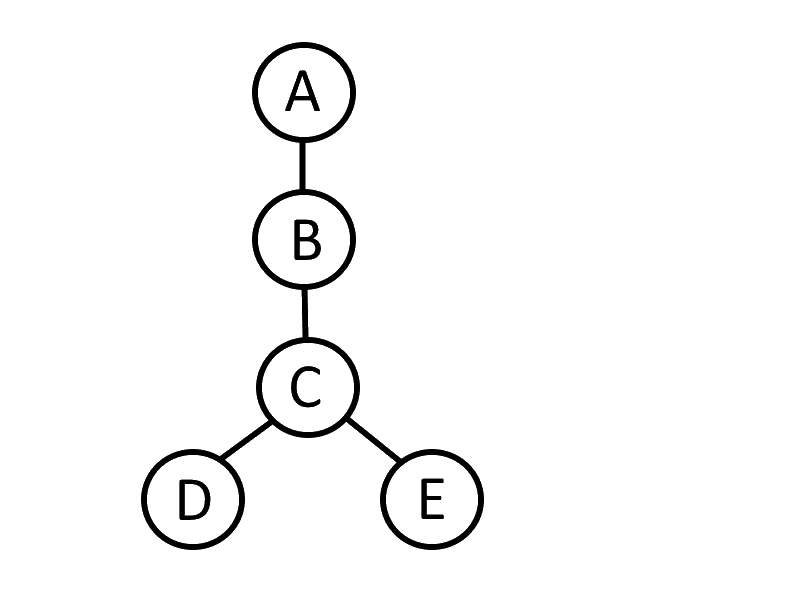
\includegraphics[width=0.4\textwidth]{betweenness_graph.png}
	\caption{A simple undirected network}
	\label{betweenness_graph}
\end{figure}

\begin{table}[!h]
	\centering
	\begin{tabular}{|c | c | c |}
		\cline{2-3}\multicolumn{1}{c|}{} 
		& 		$C_{B}(v)$	& $Normalized \; C_{B}(v)$ \\\hline 
		$A$		& 0 		& 0 						\\\hline 
		$B$ 	& 3.0		& 0.5 						\\\hline 
		$C$ 	& 5.0		& 0.8$\overline{3}$ 		\\\hline 
		$D$ 	& 0 		& 0							\\\hline 
		$E$ 	& 0 		& 0 						\\\hline 
	\end{tabular}
	\caption{An example of betweenness centrality measure calculated from Figure (\ref{betweenness_graph})}
\end{table}

Girvan-Newman algorithm calculates the betweenness using the fast algorithm of Newman \cite{ref-1, ref-13}. This calculates the betweenness for $m$ edges in a graph of $n$ vertices in time $\mathcal{O}(mn)$. To reduce the running time of the algorithm further, one might be tempted to calculate the betweenness of all the edges only once and then remove them in order of decreasing betweenness. But this strategy does not work well because if two communities are connected by more than one edge, then there is no guarantee that all of those edges will have high betweenness. In practical applications, the Girvan-Newman algorithm with betweenness centrality gives better results than adopting other centrality measures \cite{ref-12}, although Girvan-Newman algorithm cannot find overlapping communities, as each vertex is assigned to a single cluster.

\subsubsection*{Fast Algorithm of Newman}\label{sub:fastalgorithm}
To detect community structure in a sparse network faster, Newman has proposed an algorithm, known as \textit{Fast algorithm of Newman}. This algorithm is based on the idea of modularity. Given any network, the GN community structure algorithm \cite{ref-1} always produces some division of the vertices into communities, regardless of whether the network has any natural such division \cite{ref-13}. To test whether a particular division is meaningful, this algorithm defines a quality function or\textit{ modularity $Q$} as follows \cite{ref-1}.

Let $e_{ij}$ be one-half of the fraction of edges in the network that connect vertices in group $i$ to those in group $j$, so that the total fraction of such edges is $e_{ij} + e_{ji}$. The only exception will be the diagonal elements $e_{ii}$, which are equal to the fraction of edges that fall within group $i$ (with no factor of a half). Then $\sum_i e_{ii}$ is the total friction of edges that fall within groups. All other edges fall between groups. The maximum value of this sum is 1, and  a division of the network into communities is good if this quality is large, meaning it is of order 1.

Let $a_i$ be the fraction of all ends that are attached to vertices in group $i$. We can calculate $a_i$ straightforwardly by noting that $a_i = \sum_j e_{ij}$. If the ends of edges are connected together at random, the fraction of the resulting edges that connect vertices within group $i$ is $a_i^2$. We define the modularity $Q$ as:
\begin{equation}
Q = \sum\limits_i (e_{ii} - a_i^2)
\end{equation}

If a particular division gives no more within-community edges than would be expected by random chance, this modularity is $Q = 0$. Values other than 0 indicates deviations from randomness and in practice values greater than about 0.3 appear to indicate significant community structure \cite{ref-12}.

The fast algorithm of Newman starts with a state in which each vertex is a sole member of one of $n$ communities, it repeatedly joins communities together in pairs, choosing at each step the  join that results in the greatest increase (or smallest decrease) in $Q$. The process of this algorithm can be represented as a dendrogram as in Figure(\ref{dendrogram}). Since, the joining of a pair of communities between which there are no edges at all can never result in an increase in $Q$, the algorithm only considers those pairs between which there are edges, of which there will at any time be at most $m$, where $m$ is the number of edges in the graph. The change in $Q$ upon joining two communities is given by
\begin{equation}
\Delta Q = e_{ij} + e_{ji} - 2 a_i a_j = 2(e_{ij} - a_ia_j)
\end{equation}
which can clearly be calculated in constant time. There is a maximum of $n - 1$ join operations necessary to construct the complete dendrogram and hence the entire algorithm runs in time $\mathcal{O}((m + n)n)$, or $\mathcal{O}(n^2)$ on a sparse graph \cite{ref-13}.

% ================================================================================================== %

\subsection{Modularity Maximization Technique}\label{subsec:modularity_maximization}
A \textit{quality function} is a function that assigns a number to each partition of a graph. In this way, one can rank partitions based on their score given by the quality function. Partition with high scores are marked as ``good", so the one with largest score is by definition the best. Nevertheless, one should keep in mind that the question is when a partition is better than another one is ill-posed, and the answer depends on the specific concept of community and/or quality function adopted.

A quality function $Q$ is additive if there is an elementary function $q$ such that, for any partition $\mathcal{P}$ of a graph
\begin{equation}\label{quality-eq-1}
Q(\mathcal{P}) = \sum\limits_{\mathcal{C} \in \mathcal{P}} q(\mathcal{C}),
\end{equation}
where $\mathcal{C}$ is a generic cluster of partition $\mathcal{P}$. Above Eq.(\ref{quality-eq-1}) states that the quality of a partition is given by the sum of the qualities of the individual clusters. The function $q(\mathcal{C})$ could be any of the cluster fitness functions adopted.

An example of a quality function is the performance $P$, which counts the number of correctly "interpreted" pairs of vertices, i.e. two vertices belonging to the same community and connected by an edge, or two vertices belonging to different communities and not connected by an edge. The definition of performance, for a partition $\mathcal{P}$, is
\begin{equation}
P(\mathcal{P}) = \frac{\vert \{(i,j) \in E, C_i = C_j\} \vert + \vert (i,j) \notin E, C_i \neq C_j\vert}{n(n-1)/2}
\end{equation}
By definition, $0 \; \le \; P(\mathcal{P}) \; \le \; 1$ \cite{ref-6}. 

Modularity is the fraction of the edges that fall within the given groups minus the expected fraction if edged were distributed at random. the value of modularity lies in the range of $[-1/2,1)$. It is positive if the number of edges within groups exceeds the number of expected on the basis of change. For a given division of the network's vertices into some modules, modularity reflects the connection of edges within modules compared with the random distribution of links between all nodes regardless of modules. In the most common version of this concept, randomization of the edges is done so as to preserve the degree of each vertex.

Consider a graph with $n$ nodes and $m$ edges such that the graph can be partitioned into two communities using a membership variable $s$. If a node $i$ belongs to community $X$, $s_i = 1$, or if $i$ belongs to community $Y$, $s_i = -1$. Let the adjacency matrix of the network be presented by $\textbf{A}$, where $\textbf{A}_{ij} = 0$ means that there's no edge between node $i$ and $j$. On the other hand, $\textbf{A}_{ij} = 1$ means there is an edge between the two. Also for simplicity, we consider an undirected graph. Thus, $\textbf{A}_{ij} = \textbf{A}_{ji}$ \footnote{It is important to note that multiple edges may exist between two nodes, but here we asses the simplest case.}. Modularity $Q$ is then defined as the fraction of  edges that fall within group $X$ or $Y$, minus the expected number of edges within groups $X$ and $Y$ for a random graph with the same node degree distribution as the given network.

The expected number of edges shall be computed using the concept of configuration models \cite{ref-16}. The configuration model is a randomized realization of a particular network. Given a network with $n$ nodes, where each node $i$ has a node degree $k_i$, the configuration model cuts each edge into two halves, and then each half edge called a \textit{stub}, is rewired randomly with any other \textit{stub} in the network even allowing self-loops. Thus, even though the node degree distribution of the graph remains intact, the configuration model results in a completely random graph.

Let the total number of \textit{stubs} be $l_n$:

\begin{equation}
l_n = \sum\limits_i k_i = 2m
\end{equation}

Now, if we randomly select two nodes $i$ and $j$ with node degrees $k_i$ and $k_j$ respectively and rewire the stubs for these two nodes, then:
\newline\newline
\textbf{Expectation of full edges between $i$ and $j$ =$\dfrac{(Full \; edges \; between \; i \; and \; j )}{(Total \; number \; of \; rewiring \; possibilities)}$} 
\newline\newline
The total number of rewiring possible is equal to the number of \textit{stubs} remaining after choosing a particular \textit{stub}, $l_{n-1}$. For large values on $n$, $l_{n-1} \approx l_n$. Thus,
\newline\newline
\textbf{Expected number of full edges between $i$ and $j$ = $\dfrac{k_i k_j}{l_n}$}
\newline\newline

Hence, the difference between the actual number of edges between node $i$ and $j$ and the expected number of edges between them is:

\begin{center}
	$\textbf{A}_{ij} - \frac{k_i k_j}{2m}$
\end{center}

Summing over all node pairs gives the equation for modularity, $\textbf{Q}$.
\begin{equation}\label{modularity_Q}
Q = \dfrac{1}{2m} \sum\limits_{ij}\left[\textbf{A}_{ij} - \dfrac{k_i k_j}{2m}\right] \dfrac{s_i s_j + 1}{2}
\end{equation}

It is important to note that Eq.(\ref{modularity_Q}) holds good for partitioning into two communities only. Hierarchical\footnote{Partitioning into two communities, then two sub-communities further partitioned into two smaller sub-communities only to maximize \textbf{Q}.} partitioning is a possible approach to identify multiple communities in a network. Additionally, Eq.(\ref{modularity_Q}) can be generalized for partitioning a network into $n_c$ communities.
\begin{equation}
Q = \dfrac{1}{(2m)} \sum\limits_{ij}\left[\textbf{A}_{ij} - \dfrac{k_i k_j}{(2m)}\right] \delta(C_i, C_j)
\end{equation}
Where $A_ij$ represents the weight of the edge between $i$ and $j$, $k_i = \sum_j A_ij$ is the sum of the weights of the edges attached to vertex $i$, $C_i$ is the community to which vertex $i$ is assigned, the $\delta$-function $\delta(u,v)$ is 1 if $u = v$ and 0 otherwise and $m = \frac{1}{2} \sum_{ij}A_{ij}$ \cite{ref-27}.
 
Since the only contributions to the sum come from vertex pairs belonging to the same cluster, we can group these contributions together and rewrite the sum over the vertex pairs as a sum over the clusters,
\begin{equation}\label{sumoverclusters}
Q = \sum\limits_{c=1}^{n_c} \left[ \dfrac{l_c}{m} - \left( \dfrac{d_c}{2m}\right)^2\right]
\end{equation}
Here, $n_c$ is the number of clusters, $l_c$ the total number of edges joining vertices of module $c$ and $d_c$ the sum of the degrees of the vertices of $c$. In Eq.(\ref{sumoverclusters}), the first term of each sum and is the fraction of edges of the graph inside the module, whereas the second term represents the expected fraction of edges that would be there if the graph were a random graph with same expected degree of each vertex.

A nice feature of modularity is that it can be equivalently expressed both in terms of the intra-cluster edges, as in Eq.(\ref{sumoverclusters}), and in terms of the inter-cluster edges. In fact, the maximum of modularity can be expressed as:
\begin{equation}\label{modularity_Q_max}
\begin{array}{c c lc}
Q_{max} & = & \max\limits_{\mathcal{P}} \left\lbrace \sum\limits_{c=1}^{n_{c}}\left[\frac{l_{c}}{m} - \left(\frac{d_{c}}{2m}\right)^2\right]\right\rbrace \\
& = & \frac{1}{m}\max\limits_{\mathcal{P}} \left\lbrace \sum\limits_{c=1}^{n_{c}}\left[l_{c} - Ex(l_{c})\right] \right\rbrace \\
& = & - \frac{1}{m}\min\limits_{\mathcal{P}} \left\lbrace - \sum\limits_{c=1}^{n_{c}}\left[l_{c} - Ex(l_{c})\right] \right\rbrace,
\end{array}
\end{equation}
where $\max_{\mathcal{P}}$ and $\min_{\mathcal{P}}$ indicate the maximum and the minimum overall possible graph partitions $\mathcal{P}$ and Ex($l_c$) = $d_c^2/4m$ indicates the expected number of links in the cluster $c$ in the null model of modularity. By adding and subtracting the total number of edges $m$ of the graph one finally gets
\begin{equation}\label{modularity_Q_max_cut}
\begin{array}{c c lc}
Q_{max} & = & -\dfrac{1}{m} \min\limits_{\mathcal{P}}\left\lbrace \left[ \left( m - \sum\limits_{c=1}^{n_c} l_c\right) - \left( m - \sum\limits_{c=1}^{n_c} Ex(l_c)\right) \right] \right \rbrace \\
& = & - \frac{1}{m} \min\limits_{\mathcal{P}} (\vert Cut_{\mathcal{P}} \vert - ExCut_{\mathcal{P}}).
\end{array}
\end{equation}
In the last expression $\vert Cut_{\mathcal{P}} \vert = m - \sum_{c=1}^{n_c} l_c$ is the number of inter-cluster edges of partition $\mathcal{P}$, and $ExCut_{\mathcal{P}} = m - \sum_{c=1}^{n_c} Ex(l_c)$ is expected number of inter-cluster edges of the partition in modularity's null model.

\subsubsection*{Modularity Optimization }\label{sebsec:modularity-optimization}
Modularity is by far the most used and best-known quality function \cite{ref-6}. By assumption, a high value of modularity indicates good partitions. So, the partition corresponding to its maximum value on a given graph might be the best or at least a very good one. An exhaustive optimization of $Q$ is not possible, due to the huge number of ways in which it is possible to partition a graph, even when the latter is small. Besides, the true maximum is out of reach, as it has been recently proved that modularity is an NP-complete problem \cite{ref-18}, so it is probably impossible to find the solution in a time growing polynomially with the size of the graph. However, there are currently several algorithms able to find fairly good approximations of the modularity maximum in a reasonable time.


\subsection{Hierarchical Clustering}\label{sub:hierarchicalclustering}
The starting point of any \textit{hierarchical clustering} method is the definition of a similarity measure between vertices. After the measure is chosen, it computes the similarity for each pair of vertices, no matter if they are connected or not \cite{ref-6}. At the end of this process, a new $ n \times n$ matrix $X$, the \textit{similarity matrix} is produced. hierarchical clustering techniques aim at identifying groups of vertices with high similarity and can be classified into two categories:

\begin{enumerate}
	\item \textit{Agglomerative algorithms}, in which clusters are iteratively merged if their similarity is sufficiently high
	\item \textit{Divisive algorithms}, in which clusters are iteratively split by removing edges connecting vertices with low similarity
\end{enumerate}

For the scope of this section we will focus on agglomerative algorithms. This thesis will also get into Divisive algorithms as it proceeds through different other methods in a later stage. Agglomerative algorithms are bottom-up, as one starts from the vertices as separate clusters (singletons) and ends up with the graph as a unique cluster. Science clusters are merged based on their mutual similarity. It is essential to define a measure that estimates how similar clusters are out of the matrix $X$. In \textit{single-linkage clustering}, the similarity between the two groups is the minimum element $x_{ij}$, with $i$ in one group and $j$ in the other.

This whole procedure can be better illustrated with the help of \textit{dendrogram} which is a very common way to represent the hierarchical structure of graph is to draw a dendrogram, like the one in Figure (\ref{dendrogram}).

\begin{figure}[H]
	\centering
	\begin{minipage}[b]{0.5\textwidth}
		\centering
		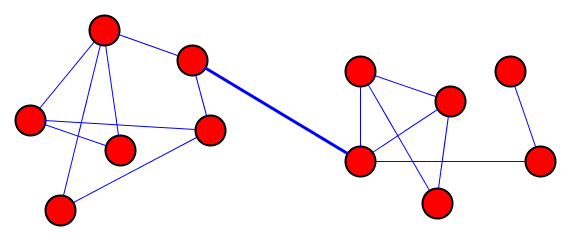
\includegraphics[width=\textwidth]{edge_betweenness.png}
		\caption{An example of edge betweenness}
		\label{edgebetweenness}
	\end{minipage}
	\begin{minipage}[b]{0.45\textwidth}
		\centering
		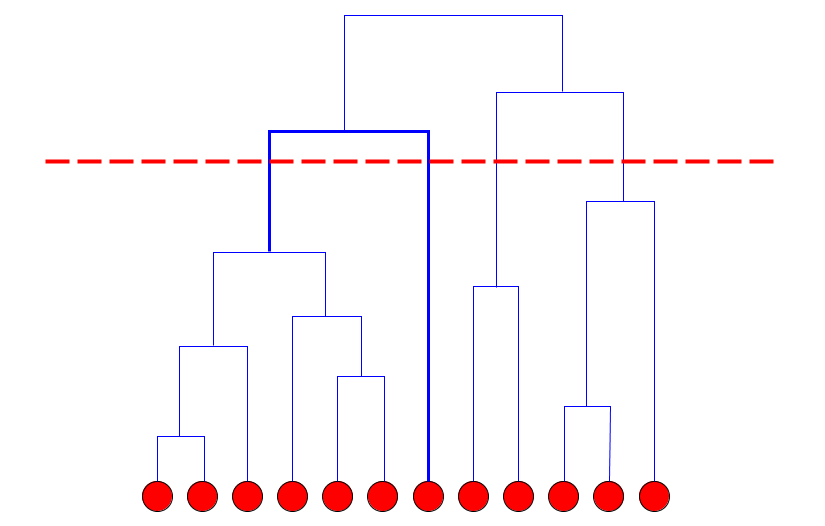
\includegraphics[width=\textwidth]{dendrogram.png}
		\caption{A dendrogram with twelve nodes from the graph in Figure (\ref{edgebetweenness})}
		\label{dendrogram}
	\end{minipage}
\end{figure}

Here, partitions of a graph with twelve vertices are shown. At the bottom, each vertex is its own module (the \textit{leaves} of the tree). By moving upwards, groups of vertices are successively aggregated. Based on the  given similarity measures \textit{mergers} of communities are represented by horizontal lines. The uppermost level represents the whole graph as a single community. Cutting the diagram horizontally at some height, as shown in the Figure (dashed line), displays one partition of the graph. The diagram is hierarchical by construction: each community belonging to a level is fully included in a community at a higher level.

Hierarchical clustering has the advantage that it does not require any preliminary knowledge on the number and size of the clusters. The result depends on the specific similarity measure adopted as described in section (\ref{vertexsimilarity}). Another problem is that vertices with just one neighbor are often classified as a separated cluster, which does not make any sense. The major weakness of agglomerative hierarchical clustering is that it does not scale well \cite{ref-6}. If points of a graph are embedded in space, so that the distance can be used as a dissimilarity measure as described in section (\ref{vertexsimilarity}), the computational complexity is $\mathcal{O}(n^2)$ for single linkage, $\mathcal{O}(n^2 \log n)$ for the complete and average linkage schemes. For graph clustering, where distance is not trivially defined, the complexity can become much heavier if the calculation of the chosen similarity measure is costly.

\subsubsection*{Vertex Similarity}\label{vertexsimilarity}
It is natural to assume that communities are groups of vertices similar to each other. The similarity between each pair of vertices with respect to some reference property, local or global, no matter whether they are connected by an edge or not can be computed. Each vertex ends up in the cluster whose vertices are most similar to it.

If it were possible to embed the graph vertices in an $n$-dimensional \textit{Euclidean space}, by assigning a position to them, one could use the \textit{distance} between a pair of vertices as a measure of their similarity \footnote{It is actually a measure of dissimilarity because similar vertices are expected to be close to each other.}. Given the two data points $A = (a_1, a_2, \dots, a_n)$ and $B = (b_1, b_2, \dots , b_n)$, one could use any norm $L_m$.\newline \newline
The \textit{Euclidean distance}($L_2$-norm):
\begin{equation}
d_{AB}^E = \sum_{k=1}^{n} \sqrt{(a_k - b_k)^2}
\end{equation}
the \textit{Manhattan distance}($L_1$-norm)
\begin{equation}
d_{AB}^M = \sum_{k=1}^{n} \vert a_k - b_k \vert
\end{equation}
and the $L_\infty$-norm will be
\begin{equation}
d_{AB}^\infty = \underset{k \in [1,n]}{\max} \vert a_k - b_k \vert
\end{equation}

Another popular spatial measure is the \textit{cosine similarity}, defined as
\begin{equation}\label{eq:cosine_similarity}
\rho_{AB} = \arccos \dfrac{\textbf{a} \cdot \textbf{b}}{\sqrt{\sum\limits_{k=1}^{n}{a_k^2}} \sqrt{\sum\limits_{k=1}^{n}{b_k^2}}}
\end{equation}
where $\textbf{a}\cdot\textbf{b}$ is the dot product of vectors \textbf{a} and \textbf{b}. The variable $\rho_{AB}$ is defined in the range $[0,\pi)$.

If the graph cannot be embedded in space, the similarity must be necessarily inferred from adjacency relationships between vertices or node properties. A possibility is to define a distance between vertices like \cite{ref-8, ref-9}.
\begin{equation}
d_{ij} = \sqrt{\sum_{k \neq {i,j}} (\textbf{A}_{ik} - \textbf{A}_{jk})^2}
\end{equation}
where \textbf{A} is the adjacency matrix. This is a dissimilarity measure, based on the concept of structural equivalence \cite{ref-10}. Two vertices are structurally equivalent if they have the same neighbors, even if they are not adjacent themselves. If $i$ and $j$ are structurally equivalent, $d_{ij} = 0$. Vertices with a large degree and different neighbors are considered very \textit{far} from each other. Alternatively, one could measure the \textit{overlap} between the neighborhoods $\varGamma(i)$ and $\varGamma(j)$ of vertices $i$ and $j$, given by the ratio between the intersection and the union of the neighborhoods, i.e.
\begin{equation}\label{eq:neihborhood-overlap}
\omega_{ij} = \dfrac{\vert \varGamma(i) \cap \varGamma(j) \vert}{\vert \varGamma(i) \cup \varGamma(j) \vert}
\end{equation}

Another very widely used measure related to structural equivalence is the \textbf{\textit{Pearson Correlation}} between columns and rows of the adjacency matrix,
\begin{equation}
C_{ij} = \dfrac{\sum\limits_{k} (A_{ik} - \mu_i) (A_{jk} - \mu_j)}{n \sigma_i \sigma_j}
\end{equation}
where the averages $\mu_i = (\sum\limits_j A_{ij} / n)$ and the variances $\sigma_i = \sqrt{\sum\limits_j (A_{ij} - \mu_i)^2} / n$

\section{Dynamic Community Detection Algorithms}\label{sec:dynamic_community_algorithms}
In section (\ref{subsub:dynamic_community}), dynamic community detection and its life cycle is described in brief. Difficulty in accessing time-stamped data for real systems represented in a graph was the main problem for dynamic community detection and observation. Until recently, availability of time-stamped graph data representing real systems lead to a path of community detection and observation, enabling to monitor the evolution of communities in time. Figure (\ref{fig:community-evolution}) illustrates the different scenarios of the community life-cycle.

The first study about community detection and observation was carried out by Hopcroft er al. in  \cite{ref-52} in 2004. Authors in this article analyzed snapshots of the citation graph data from NEC CiteSeer Database. These snapshots covered the period from 1990 to 2001. In that article, author used \textit{hierarchical clustering} (section \ref{sub:hierarchicalclustering}) to detect communities, where similarity between vertices (nodes) is the \textit{cosine similarity} (Equation \ref{eq:cosine_similarity}) of the vectors describing the corresponding papers. Authors found the best matching communities across different snapshots and in this way they were able to observe the evolution of community structures.

In 2007, Palla et al. in \cite{ref-23} performed a semantic analysis of dynamic communities. The authors used two different data-sets from two different systems. One was a year's phone call data and another one was a graph of the collaboration network between scientists, describing co-authorship of papers over 142 months. They faced a few challenges along the way to determine the best course of action to detect and observe communities over time, the first challenge was to identify the image of community $\mathcal{C}(t+1)$ at time $t+1$ among the communities of the graph at time $t$. A simple way to see the evolution of community is to see the overlap of communities between time $t$ and $t+1$. The problem is at time-stamp $t+1$, a community that existed at time-stamp $t$ might have changed and in this process, it might miss the actual evolution of the communities. Authors of \cite{ref-23}, solved the problem by using Clique Percolation Method (see \cite{ref-6} section 11.1). The general idea is to analyze a graph $\mathcal{G}(t, t+1)$, obtained by merging two snapshots $\mathcal{G}(t)$ and $\mathcal{G}(t+1)$ of evolving graph at time-stamp $t$ and $t+1$. So these, CPM communities {$\mathcal{C}^{t+1}$} has the largest relative overlap with community {$\mathcal{C}^t$} at time $t$.

Sun et al. in \cite{ref-53}, used a method of information compression called MDL (Minimum Description Length) described in \cite{ref-54} to find the minimum encoding cost for the description of a time sequence of graphs and their partitions in communities. In this method, a bipartite graph is considered and the time sequence of the graphs can be separated into segments. For each graph segment, it is possible to define encoding cost, which combines the encoding cost of the partition of the graphs of the segment with the entropy of compression of the segment in the sub-graph segments induced by the partition. The total encoding cost $C$ of the graph series is given by the sum of the encoding costs of its segment. Minimizing $C$ helps to find not only most modular partition for each graph segment, but also the most compact subdivision of the snapshots into segments \cite{ref-54}. Authors call this process \textit{Graphscope}. It has an advantage of not requiring any input parameters, like the number and sizes of the clusters. It is also suitable for operation in streaming environment, in which new graph configurations are added in time, following the evaluation of the system \cite{ref-53}.

It is mention-able that there is another approach that monitors the evolution of communities based on vertex-centric perspective. In this method, the community of a given vertex is monitored at different times. For any method given a vertex $i$ and a time $t$, the community to which $i$ belongs to at the time $t$ is well defined. Fenn et al. in \cite{ref-55} used the multi-resolution method to analyze a fully connected graph. Authors identify the role of individual vertices in their community through the pair $(z^{in}, z^b)$, where $z^{in}$ is the $z$-score of the internal strength defined in Eq. (\ref{eq:participation_ratio}) introduced by Guimera and Amaral in \cite{ref-56}, and $z^b$  is the $z$-score of the site betweenness, defined by replacing the internal degree with the site betweenness of Freeman \cite{ref-11} in Eq. (\ref{eq:participation_ratio})

\begin{equation}\label{eq:participation_ratio}
z_i = \dfrac{k_i - \bar{k}_{s_{i}}}{\sigma_{k_{s_{i}}}}
\end{equation}
where $k_i$ is the internal degree of $i$ in its cluster $s_i$, $\bar{k}_{s_{i}}$ and $\sigma_{k_{s_{i}}}$ the average and standard deviation of the internal degrees for all vertices of cluster $s_{i}$.

As a measure of persistence, Fenn et al. introduced a vertex-centric version of the relative overlap equation:

\begin{equation}
a_i^t(\tau) = \dfrac{\lvert\mathcal{C}_i(t) \cap \mathcal{C}_i(t+\tau)\rvert}{\lvert\mathcal{C}_i(t) \cup \mathcal{C}_i(t+\tau)\rvert}
\end{equation}
Where $i$ is the vertex and $\mathcal{C}_i(t)$, $\mathcal{C}_i(t+\tau)$ the communities of $i$ at times $t$, $t+\tau$ respectively. The decay of $a_i^t(\tau)$ depends on the type of vertex. In particular, if the vertex is strongly connected to its community ($z^i$ large), $a_i^t(\tau)$ decays quite slowly, meaning that it tends to stay attached to a stable core of vertices.